\documentclass[master,euler,twoside,openright]{ustcthesis}
% 默认twoside 双面打印
% 将master修改为bachelor, doctor or master
% 要使用adobe字体,添加adobefonts选项
% 使用euler数学字体,如不愿使用,去掉euler
% 使用外文写作,请添加notchinese

% 设置图形文件的搜索路径
\graphicspath{{figures/}}

%仅用于本示例文档中显示特殊字符串
\usepackage{xltxtra}

%%%%%%%%%%%%%%%%%%%%%%%%%%%%%%
%% 封面部分
%%%%%%%%%%%%%%%%%%%%%%%%%%%%%%

  % 中文封面内容
  \title{中国科学技术大学\\硕士毕业论文}%一般情况下扉页和封皮、书脊共用一个标题文本,可以不用定义\spinetitle (仅硕博有用), \covertitle(本硕博均有用)和\encovertitle(仅本科有用)。特殊情况见下。
  \spinetitle{\small{中国科学技术大学硕士毕业论文\raisebox{-3pt}{(Beta)}}}
  %特殊情况1:本例中\title命令里含有换行控制字符,这会导致制作书脊的时候出现错误,例如如果你注释掉\spinetitle{...}这一行就会报错。这时需要定义一个不含换行等命令的\spinetitle,这并不表示\spinetitle里不能有任何命令——只能使用有限的命令。
  %特殊情况2:本例中标题过长,所以需要缩小书脊标题的字号。
  %特殊情况3:本例中中英文混排,由于tex竖排的原理限制,中英文基线不重合,所以需要人工调整英文的基线。具体调整量根据不同字体有所不同。
  \covertitle{中国科学技术大学硕士毕业\\论文}
  %\covertitle{中文题目第一行\\中文题目第二行}
  %不要在此调整封皮字体大小! Do not set Cover Page font size here!
  %特殊情况4:本例中\title中含有多个换行,导致标题超过了两行。根据制本厂规定,封皮标题不能超过两行。因此需要定义封皮使用的标题\covertitle. 如果你注释掉这一行,就会发现封皮不符合规定。
  \encovertitle{USTC Thesis Master Thesis}
  %\encovertitle{English Title Line 1\\English Title Line 2\\English Title Line 3}
  %不要在此调整封皮字体大小! Do not set Cover Page font size here!
  %特殊情况5:仅本科生有用。本科封皮中有英文标题,不超过三行。与上类似。

  \author{管亚亭}
  \depart{十一系}%系别,硕博请用系代号,本科请用全称如
  %\depart{数理化和信息工程系}
  \major{计算机应用技术}%专业,硕博请用全称,本科不需要
  \advisor{刘贵全\ 副教授}
  %\coadvisor{冯晨珠\ 教授}%第二导师,没有请注释掉
  \studentid{SA13011092}%For bachelor only
  \submitdate{二〇一六年六月}

  % 英文封面内容
  \entitle{USTC Master Thesis}
  \enauthor{Yating Guan}
  \enmajor{Computer Application Technology}
  \enadvisor{Prof. Guiquan Liu}
  %\encoadvisor{Prof. Chenzhu Feng}%另外一个导师
  \ensubmitdate{April, 2016}

%%%%%%%%%%%%%%%%%%%%%%%%%%%%%%%%%%%%%%%%%%%%%%%%%%%%%%%%%%%%%%%%%%%%%
% If you use another language instead of chinese and english, then you
% should define some strings and provide information in your language.
%%%%%%%%%%%%%%%%%%%%%%%%%%%%%%%%%%%%%%%%%%%%%%%%%%%%%%%%%%%%%%%%%%%%%
%  \otherustcstr{zhong guo ke xue ji shu da xue}%A translation of `University of Science and Technology of China' in your language
%  \otherthesisstr{shuo shi xue wei lun wen}%A translation of `A dissertation for doctor(master/bachelor)'s degree' in your language
%  \otherauthorstr{xing ming}%A translation of `Author' in your language
%  \otherdepartmentstr{yuan xi}%A translation of `Department' in your language
%  \otherstudentidstr{xue hao}%A translation of `Student ID' in your language
%  \othersupervisorstr{dao shi}%A translation of `Supervisor' in your language
%  \otherfinishedtimestr{ri qi}%A translation of `Finished Time' in your language
%  \otherspecialitystr{zhuan ye}%A translation of `Speciality' in your language
%  \othertitle{zhong guo ke xue ji shu da xue tong yong xue wen lun wen shi li wen dang}
%  \otherauthor{zhao qian sun}
%  \otheradvisor{zhou wu zheng}
%  \othercoadvisor{feng chen zhu}
%  \othersubmitdate{hou nian ma yue}
%  \othermajor{mou zhuan ye}
%  \otherdepart{mou xi}

\begin{document}

  % 封面
  \maketitle

%特别注意,以下述顺序为准,在对应部分添加文档部件,切勿颠倒顺序:
%本科论文的文档部件顺序是:
%    frontmatter:致谢、目录、中文摘要、英文摘要、
%    mainmatter: 正文章节
%    backmatter: 参考文献或资料注释、附录
%硕博论文的文档部件顺序是:
%    frontmatter:中文摘要、英文摘要、目录、符号说明
%    mainmatter: 正文章节
%    backmatter: 参考文献、附录、致谢、发表论文
%%%%%%%%%%%%%%%%%%%%%%%%%%%%%%
%% 前言部分
%%%%%%%%%%%%%%%%%%%%%%%%%%%%%%
\frontmatter
\makeatletter
\ifustc@bachelor
	%%%%%%%%%%%%%%%%%
	%本科论文修改这里
	%%%%%%%%%%%%%%%%%
	% 致谢
	
\begin{thanks}

感谢原本科模板的作者XPS、硕博模板的作者刘青松以及它们的维护者的辛勤工作!

感谢大家对本模板更新工作的支持!

本模板以及本示例文档还存在许多不足之处,欢迎大家测试并及时提供反馈。

\begin{flushright}
ywg@USTC
\end{flushright}


在中国科技大学完成本科和硕博连读学业的九年里,我所从事的学习和研究工作,都是在导师以及系里其他老师和同学的指导和帮助下进行的。在完成论文之际,请容许我对他们表达诚挚的谢意。

首先感谢导师XXX教授和XXX副教授多年的指导和教诲,是他们把我带到了计算机视觉的研究领域。X老师严谨的研究态度及忘我的工作精神,X老师认真细致的治学态度及宽广的胸怀,都将使我受益终身。

感谢班主任XXX老师和XX老师多年的关怀。感谢XXX、XX、XX等老师,他们本科及研究生阶段的指导给我研究生阶段的研究工作打下了基础。

感谢XX、XXX、XXX、XX、XXX、XXX、XXX、XX等师兄师姐们的指点和照顾;感谢XXX、XX、XXX等几位同班同学,与你们的讨论使我受益良多;感谢XXX、XX、XXX、XX、XXX等师弟师妹,我们在XXX实验室共同学习共同生活,一起走过了这段愉快而难忘的岁月。

感谢科大,感谢一路走过来的兄弟姐妹们,在最宝贵年华里,是你们伴随着我的成长。

最后,感谢我家人一贯的鼓励和支持,你们是我追求学业的坚强后盾。

\vskip 18pt

\begin{flushright}

~~~~赵钱孙~~~~

\today

\end{flushright}

\end{thanks}

	
	%目录部分
	%目录
	\tableofcontents
	%默认表格、插图、算法索引名称分别为“表格索引”、“插图索引”和“算法索引”
	%如果需要自行修改lot,lof,loa的名称,请定义
	%\ustclotname{...}
	%\ustclofname{...}
	%\ustcloaname{...}

	% 表格索引
	\ustclot
	% 插图索引
	\ustclof
	%算法索引
	%如果需要使用算法环境并列出算法索引,请加入补充宏包。
	\ustcloa
	
	% 摘要
	
\begin{cnabstract}
互联网现在已成为人们日常生活中获取信息的主要途径。人们也经常习惯于用搜索引擎来获取自己需要的知识。然而随着网页元素的多样化,除去修饰和繁杂的广告,直接发现网页的正文内容,变得越来越迫切,尤其是对于想要阅读网页新闻内容的用户。为此,实现新闻网页正文内容的提取,以及新闻网页模板的生成,成为一个需要解决的重要问题。

\keywords{正文提取,模板生成,搜索引擎}
\end{cnabstract}


\begin{enabstract}

Internet has become the main way for people to release information.And people also used to get required knowledge from the Internet with search engine.However,with the  diversification of html page elements,to remove the decoration and multifarious advertisement for discovering the main content of the Web pages,is becoming more and more urgent,especially to the users who is interesting in reading news pages.In this way,realize  the extraction of the text content of news pages , as well as the news page template generation, become a important problem to be resolved. 

\enkeywords{Content Extraction,Template Generation, Search Engine}
\end{enabstract}
%此文件中含有中英文摘要
\else
	%%%%%%%%%%%%%%%%%
	%硕博论文修改这里
	%%%%%%%%%%%%%%%%%
	% 摘要
	
\begin{cnabstract}
互联网现在已成为人们日常生活中获取信息的主要途径。人们也经常习惯于用搜索引擎来获取自己需要的知识。然而随着网页元素的多样化,除去修饰和繁杂的广告,直接发现网页的正文内容,变得越来越迫切,尤其是对于想要阅读网页新闻内容的用户。为此,实现新闻网页正文内容的提取,以及新闻网页模板的生成,成为一个需要解决的重要问题。

\keywords{正文提取,模板生成,搜索引擎}
\end{cnabstract}


\begin{enabstract}

Internet has become the main way for people to release information.And people also used to get required knowledge from the Internet with search engine.However,with the  diversification of html page elements,to remove the decoration and multifarious advertisement for discovering the main content of the Web pages,is becoming more and more urgent,especially to the users who is interesting in reading news pages.In this way,realize  the extraction of the text content of news pages , as well as the news page template generation, become a important problem to be resolved. 

\enkeywords{Content Extraction,Template Generation, Search Engine}
\end{enabstract}
%此文件中含有中英文摘要
	% 目录
	\tableofcontents
	%默认表格、插图、算法索引名称分别为“表格索引”、“插图索引”和“算法索引”
	%如果需要自行修改lot,lof,loa的名称,请定义
	%\ustclotname{...}
	%\ustclofname{...}
	%\ustcloaname{...}

	% 表格索引
	\ustclot
	% 插图索引
	\ustclof
	%算法索引
	%如果需要使用算法环境并列出算法索引,请加入补充宏包。
	\ustcloa
	
	%符号说明,需要加入补充包
	\begin{denotation}

\item[HPC] 高性能计算 (High Performance Computing)
\item[cluster] 集群
\item[Itanium] 安腾
\item[SMP] 对称多处理
\item[API] 应用程序编程接口
\item[PI]	聚酰亚胺
\item[MPI]	聚酰亚胺模型化合物,N-苯基邻苯酰亚胺
\item[PBI]	聚苯并咪唑
\item[MPBI]	聚苯并咪唑模型化合物,N-苯基苯并咪唑
\item[PY]	聚吡咙
\item[PMDA-BDA]	均苯四酸二酐与联苯四胺合成的聚吡咙薄膜
\item[$\Delta G$]  	活化自由能~(Activation Free Energy)
\item [$\chi$] 传输系数~(Transmission Coefficient)
\item[$E$] 能量
\item[$m$] 质量
\item[$c$] 光速
\item[$P$] 概率
\item[$T$] 时间
\item[$v$] 速度
\end{denotation}
%不是必需的,如果不想列出请注释掉
\fi
\makeatother

%%%%%%%%%%%%%%%%%%%%%%%%%%%%%%
%% 正文部分
%%%%%%%%%%%%%%%%%%%%%%%%%%%%%%
\mainmatter

  \chapter{绪论}
\label{chap:introduction}

\section{研究背景}
\subsection{背景介绍}

  \chapter{模板的基础使用说明}

\section{模板基本说明}
使用本模板,您应首先具备基本的\LaTeX 知识,如果您刚刚接触\LaTeX,建议您先学习相关的用户文档或教程。

模板文件名为ustcthesis.cls。方便起见,将该文件放置在与论文主文件同一文件夹中即可。如果需要使用增强功能,模板提供了一个名为ustcxtra.cls的补充包。将该文件放置在与论文主文件同一文件夹中即可。

模板提供一个文档类ustcthesis,使用\verb|\documentclass{ustcthesis}|来加载模板。

模板可以使用ctexbook文档类的相应选项,默认加载的是 cs4size, a4paper, fancyhdr, fntef。需要注意的是默认加载 \emph{双面/章节从奇数页开始} 选项,如果需要\emph{单面} 选项,请使用:
\begin{Code}
\documentclass[<学位>,oneside,openany]{ustcthesis}
\end{Code}

\begin{table}[htp]
\centering
\tabcaption{模板提供的新文档选项}
\label{tab:newdocopt}
\begin{tabular}{lL{5cm}L{4cm}}
\toprule
文档选项&说明&备注\tabularnewline
\midrule
bachelor	&学士				&\multirow{3}{4cm}{指明论文类型,不能同时存在}\tabularnewline
master		&硕士				&\tabularnewline
doctor		&博士				&\tabularnewline
basic		&仅使用基础功能	&此时无法使用增强包中的命令\tabularnewline
oldfontcfg	&使用老版本的硕博论文模板的字体设置			&需要补充包\tabularnewline
euler		&使用euler数学字体&需要补充包\tabularnewline
adobefont	&使用adobe的字体	&\multirow{2}{4cm}{仅仅防止误输入}\tabularnewline
adobefonts	&使用adobe的字体	&\tabularnewline
notchinese	&使用外文撰写论文	Use this option to write thesis in other laguage(s)& If you use language(s) other than Chinese and English, you should refer to \autoref{tab:newcmd}. \tabularnewline
\bottomrule
\end{tabular}
\end{table}

\subsection{模板推荐加载设置}
推荐使用如下选项加载模板:
\begin{Code}
\documentclass[<学位>,euler,twoside,openright]{ustcthesis}
\end{Code}

如果缺少大多数宏包,建议使用
\begin{Code}
\documentclass[<学位>,basic,twoside,openright]{ustcthesis}
\end{Code}

\section{模板提供的新环境和命令}
模板提供了若干个新环境和命令,如\autoref{tab:newenv}和\autoref{tab:newcmd}所列,这些新环境和命令有的比较简单,有的则附有对应的示例。

\begin{longtable}{lll}%@{\extracolsep{\fill}}
\caption[模板提供的新环境]{模板提供的新环境}
\label{tab:newenv} \\
\toprule
名称  & 说明 & 备注\tabularnewline\midrule
\endfirsthead
\bottomrule
\endfoot
\caption[模板提供的新环境(续)]{模板提供的新环境(续)} 
\label{tab:newenv2} \\
\toprule
名称  & 说明 & 备注\tabularnewline\midrule
\endhead
\bottomrule
\endlastfoot
enabstract&英文摘要&\tabularnewline
cnabstract&中文摘要&\tabularnewline
thanks&致谢&\tabularnewline
denotation&主要符号对照表&需要ustcxtra,用法见./chapter/denotation.tex\tabularnewline
Code&代码&需要ustcxtra,效果见\autoref{codex}\tabularnewline
Codex&代码&需要ustcxtra,效果见\autoref{codex}\tabularnewline
CodeScript&代码&需要ustcxtra,效果见\autoref{codex}\tabularnewline
CodexScript&代码&需要ustcxtra,效果见\autoref{codex}\tabularnewline
code&代码&需要ustcxtra,效果未测试\tabularnewline
theorem &定理&\tabularnewline
lemma &引理&\tabularnewline
example &例&\tabularnewline
algorithm &算法&\tabularnewline
definition &定义& \tabularnewline
axiom &公理 &\tabularnewline
property &性质 & \tabularnewline
proposition &命题 &\tabularnewline
corollary& 推论 &\tabularnewline
remark &注解  &\tabularnewline
condition &条件 & \tabularnewline
conclusion &结论 & \tabularnewline
assumption &假设 & \tabularnewline
prove &证明 &\tabularnewline
proof&证明 &与prove的区别见\autoref{pic:proofandprove}\tabularnewline
\end{longtable}

\begin{longtable}{lp{0.35\textwidth}p{0.35\textwidth}}%@{\extracolsep{\fill}}
\caption[模板提供的新命令]{模板提供的新命令}
\label{tab:newcmd} \\
\toprule
名称  & 说明 & 备注\tabularnewline\midrule
\endfirsthead
\bottomrule
\endfoot
\caption[模板提供的主要新命令(续)]{模板提供的主要新命令(续)} 
\label{tab:newcmd2} \\
\toprule
名称  & 说明 & 备注\tabularnewline\midrule
\endhead
\bottomrule
\endlastfoot
\textbackslash chuhao\{\}&字号:初号&类似的有:\textbackslash yihao\{\}...\textbackslash qihao\{\}\tabularnewline
\textbackslash xiaochu\{\}&字号:小初号&类似的有:\textbackslash xiaoer\{\}...\textbackslash xiaowu\{\}\tabularnewline
\textbackslash xiaochuhao\{\}&字号:小初号&类似的有:\textbackslash xiaoerhao\{\}...\textbackslash xiaowuhao\{\}\tabularnewline
\textbackslash ustclofname\{\}&定义图表索引名称&需在\textbackslash ustclof前使用\tabularnewline
\textbackslash ustclof&生成图表索引并加入目录&\tabularnewline
\textbackslash ustclotname\{\}&表格索引名称&与\textbackslash ustclofname\{\}类似\tabularnewline
\textbackslash ustclot&表格索引&与\textbackslash ustclot类似\tabularnewline
\textbackslash ustcloaname\{\}&算法索引名称&需要ustcxtra,与\textbackslash ustclofname\{\}类似\tabularnewline
\textbackslash ustcloa&算法索引&需要ustcxtra,与\textbackslash ustclof类似\tabularnewline
\textbackslash title\{\}&标题&中文\tabularnewline
\textbackslash author\{\}&作者&中文\tabularnewline
\textbackslash advisor\{\}&导师&中文\tabularnewline
\textbackslash coadvisor\{\}&第二导师&中文,可留空\tabularnewline
\textbackslash major\{\}&专业&硕博全称,本科不需要\tabularnewline
\textbackslash depart\{\}&院系&硕博代号,本科全称\tabularnewline
\textbackslash submitdate\{\}&完成日期&中文\tabularnewline
\textbackslash en...\{\}&由title至submitdate&以上命令的英文版本\tabularnewline
\textbackslash studentid\{\}&学号&仅本科需要\tabularnewline
\textbackslash spinetitle\{\}&书脊使用的标题&在\textbackslash title中含有部分控制命令时使用\tabularnewline
\textbackslash covertitle\{\}&封皮使用的中文标题&在\textbackslash title超过两行或其他情况时使用\tabularnewline
\textbackslash coverentitle\{\}&封皮使用的英文标题&仅本科需要,在\textbackslash entitle超过三行或其他情况时使用\tabularnewline
\textbackslash makecover[][]&生成制本厂规定格式的封皮&详细用法见main.tex文件中注释\tabularnewline
\textbackslash keywords\{\}&中文关键词&在cnabstract中使用\tabularnewline
\textbackslash enkeywords\{\}&英文关键词&在enabstract中使用\tabularnewline
\textbackslash figcaption\{\}&图形标题&无论是否在图形环境中均可得到正确标题\tabularnewline
\textbackslash tabcaption\{\}&&与上类似,表格用\tabularnewline
C\{width\}&定宽居中&表格环境中p\{width\}的加强,参考\autoref{tab:tblcmp}\tabularnewline
L\{width\}&定宽左齐&\tabularnewline
R\{width\}&定宽右齐&\tabularnewline
\textbackslash scite\{\}&上标引用&\tabularnewline
\textbackslash song&宋体&另有其他,详见ustcxtra\tabularnewline
\textbackslash upGamma&立直希腊Gamma&另有其他,详见ustcxtra\tabularnewline

\textbackslash otherustcstr  & 'University of Science and Technology of China'. A translation of this string in your own language. \emph{Only useful when you are writting a thesis in language(s) other than Chinese and English}. &  According to regulations of USTC, your need to put three title pages: Chinese, English and your own language title pages. So use these commands to generate the third title page. \tabularnewline%
\textbackslash otherthesisstr  & 'A dissertation for bachelor(/master/doctor)'s degree' & Similar to previous one \tabularnewline%
\textbackslash otherauthorstr  & 'Author' & Similar to previous one \tabularnewline%
\textbackslash otherdepartmentstr  & 'Department' & Similar to previous one \tabularnewline%
\textbackslash otherstudentidstr  & 'Student ID' & Similar to previous one \tabularnewline%
\textbackslash othersupervisorstr  & 'Supervisor' & Similar to previous one \tabularnewline%
\textbackslash otherfinishedtimestr  & 'Finished Time' & Similar to previous one \tabularnewline%
\textbackslash otherspecialitystr  & 'Speciality' & Similar to previous one \tabularnewline%
\textbackslash othertitle  & Thesis title. Put your thesis title in your own language here. \emph{Only useful when you are writting a thesis in language(s) other than Chinese and English}. &   \tabularnewline
\textbackslash otherauthor  & Your name & Similar to previous one \tabularnewline
\textbackslash otheradvisor  & Your advisor's name & Similar to previous one \tabularnewline
\textbackslash othercoadvisor  & Co-advisor & Similar to previous one \tabularnewline
\textbackslash othersubmitdate  & Thesis submit date & Similar to previous one \tabularnewline
\textbackslash othermajor  & Your major & Similar to previous one \tabularnewline
\textbackslash otherdepart  & Your department & Similar to previous one \tabularnewline
\end{longtable}

需要注意的是,这里prove环境翻译为“证明”,事实上,其实prove环境不是用作theorem等类似环境配套证明的,prove环境是与theorem等环境同级别的环境。与theorem等环境相配套的证明环境是proof环境。使用时请注意下两个环境的差异:proof环境是没有编号的,是与theorem这类环境配合使用的;prove环境是有编号的,更多的是类似于证明题的题目。详细的差别见\autoref{pic:proofandprove}。

\begin{figure}
\centering
  \framebox{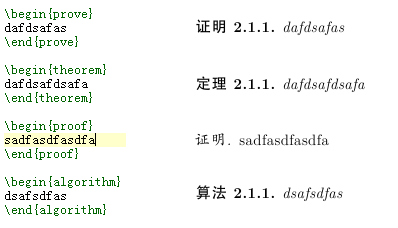
\includegraphics[scale=1]{figures/proofandprove}}
  \figcaption{proof、prove以及部分其他数学环境的差异}
  \label{pic:proofandprove}
\end{figure}

\section{使用模板的一些建议}

公式、章节、图和表格等(不包括脚注和参考文献)的交叉引用可以使用\verb|\autoref{label}|来得到正确的引用。例如使用\verb|\autoref{some_pic}|可以得到“图 X”的引用,使用\verb|\autoref{some_table}|可以得到“表 X”的引用。

建议使用\verb|\figcaption{}|命令得到所有图形的标题,表格也是。这样无论是否在图形环境中均能够得到正确的带图/表编号的标题,而在图形环境之外使用\verb|\caption{}|命令会报错。

%封面是按照制本厂的要求制作的,其中行宽和行高都是固定的,中文标题最多占两行,英文标题最多占三行。如果您的题目超过了这个限制,请缩减题目长度,不要擅自修改模板中的相关配置参数。


  
\chapter{代码示例}
\label{chap:example}
\section{Euler数学字体示例}
$$
abcdefghijklmnopqrstuvwxyz
$$
$$
ABCDEFGHIJKLMNOPQRSTUVWXYZ
$$
$$
0123456789
$$
\begin{equation}
\begin{split}
\{S_i=0\}=\frac{a_i}{b_i+a_i} \\
\{S_i=1\}=\frac{b_i}{b_i+a_i} \label{1}
\end{split}
\end{equation}

\section{上标引用示例}
\verb|\scite{lshort-cn}|,效果\scite{lshort-cn}。

\section{表格环境加强命令示例}
本模板提供了表格环境下p\{width\}加强版命令,使用L\{width\}等可以在指定宽度的同时指定对齐方式。

\begin{minipage}{\textwidth}
\begin{Codex}[numbers=left]
\begin{table}
\tabcaption{几种命令效果对比的对比}
\label{tab:tblcmp}
\centering
\begin{tabular}{c||l|c|r|p{2.5cm}|L{2.5cm}|C{2.5cm}|R{2.5cm}}
\hline
命令&l&c&r&p\{width\}&L\{width\}&C\{width\}&R\{width\}\\
\hline
效果&左齐&居中&右齐&定宽&左齐定宽&居中定宽&右齐定宽\\
\hline
\end{tabular}
\end{table}
\end{Codex}

\tabcaption{几种命令效果对比的对比}
\label{tab:tblcmp}
\centering
\begin{tabular}{c||l|c|r|p{2.5cm}|L{2.5cm}|C{2.5cm}|R{2.5cm}}
\hline
命令&l&c&r&p\{width\}&L\{width\}&C\{width\}&R\{width\}\\
\hline
效果&左齐&居中&右齐&定宽&左齐定宽&居中定宽&右齐定宽\\
\hline
\end{tabular}
\end{minipage}

\section{自定义代码环境示例}
\label{codex}
\subsection{Code环境}
\begin{minipage}{\textwidth}
\begin{minipage}{0.4\textwidth}
\begin{Code}[label=a.cpp, numbers=left]
This is Code environment
A simple example.
For more options, see fancyvrb's manual.
\end{Code}
\end{minipage}
\hfill\begin{minipage}{0.4\textwidth}
\begin{Verbatim}[fontsize=\scriptsize,baselinestretch=0.9,xleftmargin=3mm,frame=lines,labelposition=all,framesep=5pt]
\begin{Code}[label=a.cpp, numbers=left]
This is Code environment
A simple example.
For more options, see fancyvrb's manual.
\end{Code}
\end{Verbatim}
\end{minipage}
\end{minipage}

\subsection{Codex环境}
\begin{minipage}{\textwidth}
\begin{minipage}{0.4\textwidth}
\begin{Codex}[label=a.cpp, numbers=left]
This is Codex environment
A simple example.
For more options, see fancyvrb's manual.
\end{Codex}
\end{minipage}
\hfill\begin{minipage}{0.4\textwidth}
\begin{Verbatim}[fontsize=\scriptsize,baselinestretch=0.9,xleftmargin=3mm,frame=lines,labelposition=all,framesep=5pt]
\begin{Codex}[label=a.cpp, numbers=left]
This is Codex environment
A simple example.
For more options, see fancyvrb's manual.
\end{Codex}
\end{Verbatim}
\end{minipage}
\end{minipage}

\subsection{CodeScript环境}
\begin{minipage}{\textwidth}
\begin{minipage}{0.4\textwidth}
\begin{CodeScript}[label=a.cpp, numbers=left]
This is CodeScript environment
A simple example.
For more options, see fancyvrb's manual.
\end{CodeScript}
\end{minipage}
\hfill\begin{minipage}{0.4\textwidth}
\begin{Verbatim}[fontsize=\scriptsize,baselinestretch=0.9,xleftmargin=3mm,frame=lines,labelposition=all,framesep=5pt]
\begin{CodeScript}[label=a.cpp, numbers=left]
This is CodeScript environment
A simple example.
For more options, see fancyvrb's manual.
\end{CodeScript}
\end{Verbatim}
\end{minipage}
\end{minipage}

\subsection{CodexScript环境}
\begin{minipage}{\textwidth}
\begin{minipage}{0.4\textwidth}
\begin{CodexScript}[label=a.cpp, numbers=left]
This is CodexScript environment
A simple example.
For more options, see fancyvrb's manual.
\end{CodexScript}
\end{minipage}
\hfill\begin{minipage}{0.4\textwidth}
\begin{Verbatim}[fontsize=\scriptsize,baselinestretch=0.9,xleftmargin=3mm,frame=lines,labelposition=all,framesep=5pt]
\begin{CodexScript}[label=a.cpp, numbers=left]
This is CodexScript environment
A simple example.
For more options, see fancyvrb's manual.
\end{CodexScript}
\end{Verbatim}
\end{minipage}
\end{minipage}

\section{表格示例}
具体代码请参考源文件./chapter/chap-example.tex。
\begin{table}[htbp]
\centering
\caption{基于因子分析的失配补偿结果}
\label{tab:jfa-gmm-ubm}
\begin{tabular}{cccccc}
    \toprule
    &\multirow{2}{*}{\#Mix}&\multicolumn{2}{c}{No-norm}
    &\multicolumn{2}{c}{Tnorm}\\
    \cline{3-4} \cline{5-6}
		&		& EER(\%) 	& MinDCF & EER(\%) 	& MinDCF\\
    \midrule
	\multirow{3}{*}{GMM-UBM}
    &256 		& 12.43 	& 0.0647	& 12.85    & 0.0580\\
    &512 		& 10.02 	& 0.0464	& 8.88 	   & 0.0370\\
    &1024 		& 9.97 	    & 0.0457	& 8.72 	   & 0.0372\\
    \midrule
	\multirow{3}{*}{Factor Analysis}
    &256 		& 8.09 	& 0.0331 	& 7.39 	& 0.0319\\
    &512 		& 7.08 	& 0.0305 	& 6.53 	& 0.0292\\
    &1024 		& 6.83 	& 0.0295 	& \textbf{6.29} 	& \textbf{0.0279}\\
 \bottomrule
\end{tabular}
\end{table}

\section{算法示例}
具体代码请参考源文件./chapter/chap-example.tex。
\IncMargin{1em}
\begin{algorithm}
\SetKwData{Left}{left}\SetKwData{This}{this}\SetKwData{Up}{up}
\SetKwFunction{Union}{Union}\SetKwFunction{FindCompress}{FindCompress}
\SetKwInOut{Input}{input}\SetKwInOut{Output}{output}
\Input{$O_t,UBM,U$}
\Output{$x,y$}
\BlankLine
\emph{$y\leftarrow 0;$$x_h\leftarrow 0;$$h=1,...,H$ }\;
\For{$i=1$ \KwTo Number of E-M iterations}{
\emph{E Step}:\\
\For{$h=1$ \KwTo $H$}{\label{forins}
对于每一条语音段,计算其EM统计量(零阶统计量$N_h$,一阶统计量$S_{X,h}$\;
}
计算每一个人所有语音段的零阶统计量$N$\\
计算每一个人所有语音段的一阶统计量$S$\\
\emph{M Step}:\\
\For{$j=1$ \KwTo Number of Gauss-Seidel iterations}{
\For{$h=1$ \KwTo $H$}{\label{forins}
估计每一语音段$h$的失配因子$x_h$
}
估计模型的话者因子$y$
}
}
\Return{$\mu = m+Dy$}
\caption{disjoint decomposition}\label{algo_disjdecomp}
\end{algorithm}\DecMargin{1em}

\section{引用参考文献示例}
参考文献测试:\citep{deng:01a}
  %自行添加
  %\include{chapter/...}

%%%%%%%%%%%%%%%%%%%%%%%%%%%%%%
%% 附件部分
%%%%%%%%%%%%%%%%%%%%%%%%%%%%%%
\backmatter

  % 参考文献
  % 使用 BibTeX
  % 选择参考文献的排版格式。注意ustcbib这个格式不保证完全符合要求,请自行决定是否使用
  \bibliographystyle{ustcbib}%{GBT7714-2005NLang-UTF8}
  \bibliography{bib/tex}
  \nocite{*} % for every item
  % 不使用 BibTeX
  % %\renewcommand{\baselinestretch}{0.5}
\begin{thebibliography}{10}

\bibitem{deng:01a}
{邓建松,~彭冉冉,~陈长松邓建松,~彭冉冉,~陈长松邓建松,~彭冉冉,~陈长松邓建松,~彭冉冉,~陈长松邓建松,~彭冉冉,~陈长松邓建松,~彭冉冉,~陈长松邓建松,~彭冉冉,~陈长松邓建松,~彭冉冉,~陈长松邓建松,~彭冉冉,~陈长松邓建松,~彭冉冉,~陈长松邓建松,~彭冉冉,~陈长松}.
\newblock {\em \LaTeXe{}~科技排版指南}.
\newblock 科学出版社,~书号:~7-03-009239-2/TP.1516, 北京, 2001.

\bibitem{wang:00a}
王磊.
\newblock {\em \LaTeXe{}~插图指南}.
\newblock 2000.

\bibitem{zhang:03a}
张林波.
\newblock {\em 关于新版~CCT~的说明}.
\newblock 2003.

\bibitem{lshort-cn}
C\TeX{} 翻译小组.
\newblock {\em lshort~中文版~3.20}.
\newblock 2003.

\bibitem{knuth86e}
Donald~E. Knuth.
\newblock {\em Computer Modern Typefaces}, volume~E of {\em Computers and
  Typesetting}.
\newblock Addison-Wesley, Reading, Massachusetts, 1986.

\bibitem{knuth86d}
Donald~E. Knuth.
\newblock {\em {METAFONT}: The Program}, volume~D of {\em Computers and
  Typesetting}.
\newblock Addison-Wesley, Reading, Massachusetts, 1986.

\bibitem{knuth86c}
Donald~E. Knuth.
\newblock {\em The {METAFONT}book}, volume~C of {\em Computers and
  Typesetting}.
\newblock Addison-Wesley, Reading, Massachusetts, 1986.

\bibitem{knuth86b}
Donald~E. Knuth.
\newblock {\em {TeX}: The Program}, volume~B of {\em Computers and
  Typesetting}.
\newblock Addison-Wesley, Reading, Massachusetts, 1986.

\bibitem{knuth86a}
Donald~E. Knuth.
\newblock {\em The {TeX}book}, volume~A of {\em Computers and Typesetting}.
\newblock Addison-Wesley, Reading, Massachusetts, 1986.

\bibitem{lamport85a}
Leslie Lamport.
\newblock {\em {LaTeX} --- A Document Preparation System: User's Guide and
  Reference Manual}.
\newblock Addison-Wesley, Reading, Massachusetts, 2nd edition, 1985.

\end{thebibliography}


  % 附录,没有请注释掉
  \begin{appendix}
    
\chapter{关于硕士、博士学位论文撰写要求}
\label{chap:requires}

学位论文是学位申请者为申请学位而撰写的学术论文,它集中作者在研究工作中获得可行的发明、理论和见解,是评判学位申请人学术水平的重要依据和获得学位的必要条件之一,也是科研领域中的主要文献资料和社会宝贵财富。
为提高研究生学位论文的质量,做到学位论文在内容和格式上规范化与统一化,特作如下规定:

\section{对学位论文的基本要求}

\textbf{一下文字仅作示例,一切以学校规定为准!}

\subsection{硕士学位论文}

根据《中华人民共和国学位条例暂行实施办法》第八条的规定,硕士学位论文应能表明作者确已在本门学科上掌握了坚实的基础理论和系统的专门知识,并对所研究的课题有新的见解,有从事科学研究或独立担负专门技术工作的能力。硕士学位论文工作一般是在硕士生完成培养计划规定的课程学习后开始,其工作内容因学科的性质不同而有所差异,一般包括文献阅读、开题报告、拟定并实施工作计划、科研调查、实验研究、理论分析和文字总结等工作。论文正文一般应不少于3万字。硕士学位论文必须有一定的工作量,在论文题目确定后,用于论文工作的时间一般不应少于1.5年。

\subsection{博士学位论文}

根据《中华人民共和国学位条例暂行实施办法》第十三条的规定,博士学位论文应能表明作者确已在本门学科上掌握了坚实宽广的基础理论和系统深入的专门知识,具有独立从事科学研究工作的能力,并在科学或专门技术工作上做出了创造性的成果。博士学位论文工作是攻读博士学位研究生培养的最重要环节,其工作时间一般应不少于2学年。博士生入学后在导师指导下明确科研方向,收集资料,阅读文献,进行调查研究,确定研究课题。一般在第二至第三学期通过开题报告并制定论文工作计划。博士生应根据论文工作计划分阶段在教研室、学术会议上报告科研和论文工作的进展情况。论文正文一般应不少于5万字。博士生用于论文研究和撰写学位论文的时间一般应不得少于2年。

特别应注意,学位论文应是本人的研究成果,在导师指导下独立完成,不得抄袭或剽窃他人成果。论文应反映作者较好地掌握了本学科、专业的研究方法和技能,学术观点必须言之有理、持之有据,论文内容应层次分明,数据可靠,文字简炼,推理严谨,立论正确。

\section{对学位论文的格式要求}

\subsection{编写要求}

硕士、博士学位论文一般应由以下全部或某几部分组成,依次为:封面、中文摘要、英文摘要 、目录、符号说明、正文、参考文献、附录、附图表、致谢、攻读学位期间发表的学术论文目录。

具体要求如下:

\subsubsection{封面}

采用研究生院规定的统一封面,封面上填写论文题目、作者姓名、导师姓名、学科(专业) 、论文完成时间。上述内容也应在扉页上填写清楚。论文题目采用黑体26磅加粗居中,其他采用宋体16磅居中。书脊用黑体12磅,上方写论文题目,中间写系别,下方写研究生姓名(彩色封面在制信厂或印刷厂装订)。

\subsubsection{论文摘要}

学位论文的中文摘要应以最简洁的语言介绍论文的概要、作者的突出论点、新见解或创造性成果。硕士学位论文中文摘要一般应在500字左右,博士学位论文中文摘要一般在1500字左右。英文摘要(Abstract)内容应与中文摘要基本相对应,要语句通顺,语法正确,能正确概括文章的内容。摘要标题采用黑体16磅居中,正文采用宋体12磅(英文用Times New Roman体12磅),行距20磅。

\subsubsection{正文}

正文是学位论文的主体和核心部分,它是将学习、研究和调查过程中筛选、观察和测试所获得的材料,经过加工整理和分析研究,由材料而形成论点。不同学科、专业有着不同的写作内容,但作为一般要求,论据、论点应力求准确、完备、清晰、通顺,实事求是,客观真切,简短精炼,合乎逻辑。一般标题字体采用黑体14磅,多级标题可采用粗体14磅或粗体12磅。正文字体采用宋体12磅(英文用Times New Roman体12磅),两端对齐书写,行距20磅。


绪论或引言是学位论文主体部分的开端,主要说明研究工作的缘起、沿革、目的、涉及范围 、国内外研究现状、相关领域的前人研究成果和知识空白、理论分析的依据、研究设想、研究方法和实际设计的概述,以及文中拟解决的问题、理论意义和实用价值等,应言简意赅,不要与摘要雷同或成为摘要的解释,也不是提要。

结论是学位论文最终和总体的结论,是整篇论文的归宿,应明确、精炼、完整、准确。要着重阐述作者研究的创造性成果、新见解、新发现和新发展,及其在本研究领域中的地位、作用、价值和意义,还可进一步提出需要讨论的问题和建议。学位论文中的计量单位、制图、制表、公式规范、缩略词和符号必须遵循GB 3100~3102—93(国家技术监督局1993-12-27发布,1994-07-01实施)有关量和单位的规定。如无标准可循,应采用本学科或专业有关权威性机构或学术团体所公布的规定。如不得已必需引用某些未公知公用的、不易为同行读者所理解的或系作者自行拟定的符合、记号、缩略词等,均应一一在第一次出现时加以说明,给以明确的定义。

\subsubsection{参考文献}

参考文献应按文中引用的顺序列出,可以分列在各章末尾,也可以列在正文的末尾。

本着以严谨求实的科学态度撰写论文,凡学位论文中有引用他人成果之处,均应详细列出所引文献的名称、作者、发表刊物、发表时间、卷号、页码等。标题字体采用黑体14磅,正文字体采用宋体10磅(英文用Times New Roman体10磅),行距16磅。

\subsubsection{附录}
主要列入正文内过分冗长的公式推导,供查读方便所需的辅助性数学工具或表格,重复性数据图表,论文使用的缩写,程序全文及说明等。

\subsubsection{致谢}

表达作者对完成论文和学业提供帮助的老师、同学、领导、同事及亲属的感激之情。

\subsubsection{攻读学位期间发表的学术论文目录}

按学术论文发表的时间顺序,列齐本人在攻读学位期间发表或已录用的学术论文清单(发表刊物名称、卷册号、页码、年月及论文署名、作者排序)。

\subsection{打印}

按照有关规定,凡授予中华人民共和国学位者,学位论文必须用中文撰写,同时一律用A4标准纸打印输出,一般应有篇眉。篇眉和页码均采用宋体10磅居中,页面设置上边距3.8cm、下边距为3.0cm,左边距为3.5cm、右边距为3.0cm。

\subsection{装订}

学位论文撰写完成后,用研究生院统一封面线装订成册。所需份数由研究生本人及导师掌握(可参考学位申请上报材料清单的要求)。

  \end{appendix}

  \makeatletter
  \ifustc@bachelor\relax\else
    % 致谢
	
\begin{thanks}

感谢原本科模板的作者XPS、硕博模板的作者刘青松以及它们的维护者的辛勤工作!

感谢大家对本模板更新工作的支持!

本模板以及本示例文档还存在许多不足之处,欢迎大家测试并及时提供反馈。

\begin{flushright}
ywg@USTC
\end{flushright}


在中国科技大学完成本科和硕博连读学业的九年里,我所从事的学习和研究工作,都是在导师以及系里其他老师和同学的指导和帮助下进行的。在完成论文之际,请容许我对他们表达诚挚的谢意。

首先感谢导师XXX教授和XXX副教授多年的指导和教诲,是他们把我带到了计算机视觉的研究领域。X老师严谨的研究态度及忘我的工作精神,X老师认真细致的治学态度及宽广的胸怀,都将使我受益终身。

感谢班主任XXX老师和XX老师多年的关怀。感谢XXX、XX、XX等老师,他们本科及研究生阶段的指导给我研究生阶段的研究工作打下了基础。

感谢XX、XXX、XXX、XX、XXX、XXX、XXX、XX等师兄师姐们的指点和照顾;感谢XXX、XX、XXX等几位同班同学,与你们的讨论使我受益良多;感谢XXX、XX、XXX、XX、XXX等师弟师妹,我们在XXX实验室共同学习共同生活,一起走过了这段愉快而难忘的岁月。

感谢科大,感谢一路走过来的兄弟姐妹们,在最宝贵年华里,是你们伴随着我的成长。

最后,感谢我家人一贯的鼓励和支持,你们是我追求学业的坚强后盾。

\vskip 18pt

\begin{flushright}

~~~~赵钱孙~~~~

\today

\end{flushright}

\end{thanks}
%硕博致谢部分
    % 发表文章目录
    
\chapter{在读期间发表的学术论文与取得的研究成果}

\noindent\textbf{研究工作:}

\begin{enumerate}

\item A A A A A A A A A
\item A A A A A A A A A
\item A A A A A A A A A
\item A A A A A A A A A

\end{enumerate}


\noindent\textbf{已发表论文:}

\begin{enumerate}

\item A A A A A A A A A 
\item A A A A A A A A A
\item A A A A A A A A A
\item A A A A A A A A A
\item A A A A A A A A A
\item A A A A A A A A A
\item A A A A A A A A A
\item A A A A A A A A A

\end{enumerate}

\vskip 1cm

\noindent\textbf{待发表论文:}

\begin{enumerate}

\item A A A A A A A A A

\end{enumerate} 
  \fi
  \makeatother

\end{document}
